\documentclass{beamer}
\usetheme{default}
\usepackage{booktabs}
\usepackage{tikz}
\usetikzlibrary{positioning}
\setbeamertemplate{navigation symbols}{}
\setbeamertemplate{footline}[frame number]

\title{Multilayer Perceptron for Classification of Mobile Price Range using Kaggle Dataset}
\author{Yusuf Imantaka Bastari - 24/532731/PA/22530}
\begin{document}
\begin{frame}[plain]
    \maketitle
\end{frame}

\begin{frame}
    \frametitle{Group Members}
    \begin{enumerate}
        \item Yusuf Imantaka Bastari - 24/532731/PA/22530
        \item \textbf{[TODO: member name - NIM]}
        \item \textbf{[TODO: member name - NIM]}
    \end{enumerate}
\end{frame}

\begin{frame}
    \frametitle{Job Description for each member}
    \begin{table}
        \centering
        \begin{tabular}{ll}
            \toprule
            Member & Job description \\
            \midrule
            Yusuf Imantaka Bastari & \textbf{[TODO]} \\
            \textbf{[TODO]} & \textbf{[TODO]} \\
            \textbf{[TODO]} & \textbf{[TODO]} \\
            \bottomrule
        \end{tabular}
    \end{table}
\end{frame}

\begin{frame}
    \frametitle{Problem Case}
    \begin{columns}[T]
        \begin{column}{0.55\textwidth}
            \begin{itemize}
                \item Kaggle \textit{Mobile Price Classification} dataset
                \item Predict the phone \texttt{price\_range} (0--3) from its specifications
                \item 2000 samples, 20 numerical features (e.g.\ \texttt{ram}, \texttt{battery\_power}, \texttt{px\_height})
                \item No missing values, no duplicates
                \item 4 balanced classes (500 samples each)
                \item Main metric: \textbf{macro F1-score}
            \end{itemize}
        \end{column}
        \begin{column}{0.45\textwidth}
            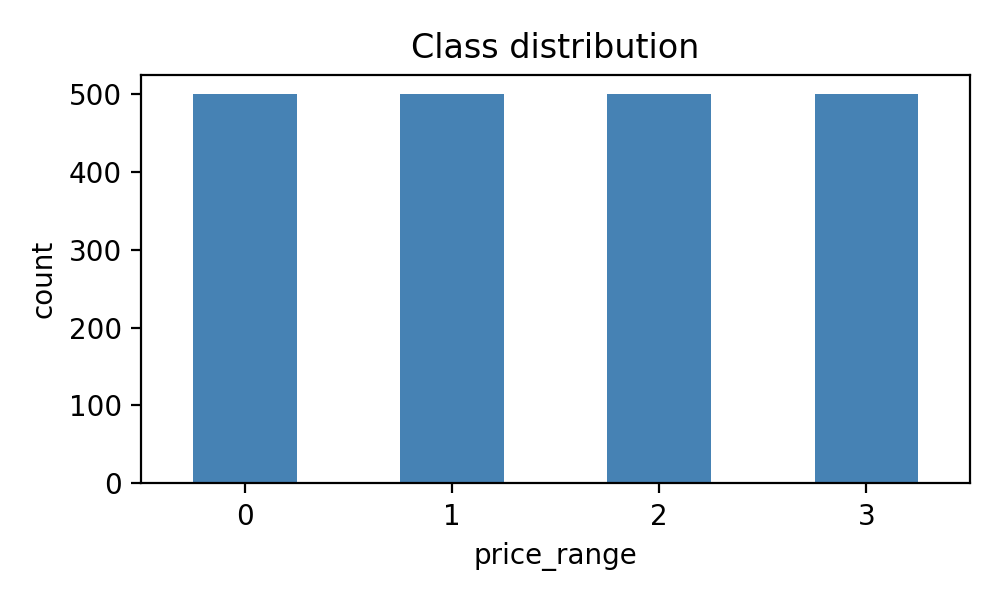
\includegraphics[width=\linewidth]{figures/class_distribution.png}
        \end{column}
    \end{columns}
\end{frame}

\begin{frame}
    \frametitle{Solution Methodology}
    \begin{enumerate}
        \item Standardize the features (fit on the training folds only, to avoid leakage)
        \item Evaluate with \textbf{stratified 5-fold cross-validation}
        \item Train a Multilayer Perceptron (MLP) classifier in PyTorch
        \item Ablation study on network layers: dropout, activation function, batch normalization
        \item Ablation study on loss functions
        \item Compare all experiments using the mean macro F1-score over the 5 folds
    \end{enumerate}
\end{frame}

\begin{frame}
    \frametitle{Neural Network Architecture}
    \begin{center}
    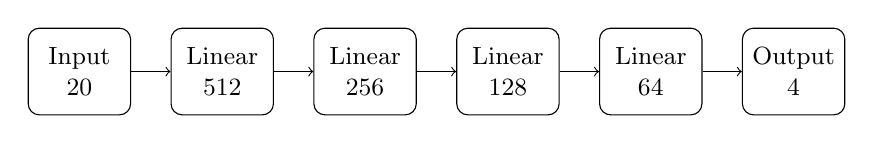
\begin{tikzpicture}[node distance=0.5cm, every node/.style={font=\small},
        box/.style={draw, rounded corners, minimum height=1.1cm, minimum width=1.3cm, align=center}]
        \node[box] (in) {Input\\20};
        \node[box, right=of in] (h1) {Linear\\512};
        \node[box, right=of h1] (h2) {Linear\\256};
        \node[box, right=of h2] (h3) {Linear\\128};
        \node[box, right=of h3] (h4) {Linear\\64};
        \node[box, right=of h4] (out) {Output\\4};
        \foreach \a/\b in {in/h1, h1/h2, h2/h3, h3/h4, h4/out} \draw[->] (\a) -- (\b);
    \end{tikzpicture}
    \end{center}
    \begin{itemize}
        \item Fully connected MLP with 4 hidden layers: $20 \rightarrow 512 \rightarrow 256 \rightarrow 128 \rightarrow 64 \rightarrow 4$
        \item Activation after every hidden layer (baseline: ReLU)
        \item Optional batch normalization (after linear) and dropout (after activation)
        \item Output: 4 logits, one per price range
    \end{itemize}
\end{frame}

\begin{frame}
    \frametitle{Learning Strategy and Parameter Tuning}
    \begin{columns}[T]
        \begin{column}{0.5\textwidth}
            \textbf{Fixed training setup}
            \begin{itemize}
                \item Optimizer: Adam
                \item Learning rate: 0.001
                \item Batch size: 64
                \item Epochs: 20
                \item Seed: 42 (same for every experiment)
                \item Stratified 5-fold, shuffled
            \end{itemize}
        \end{column}
        \begin{column}{0.5\textwidth}
            \textbf{Tuned by ablation}
            \begin{itemize}
                \item Layers: dropout (0.2, 0.5); ReLU, LeakyReLU, ELU, GELU, Tanh; batch norm
                \item Loss: cross-entropy, label smoothing (0.1), focal ($\gamma=2$), multi-margin, MSE on one-hot
            \end{itemize}
        \end{column}
    \end{columns}
\end{frame}

\begin{frame}
    \frametitle{Results Experiment: Network Layers}
    \begin{columns}[c]
        \begin{column}{0.62\textwidth}
            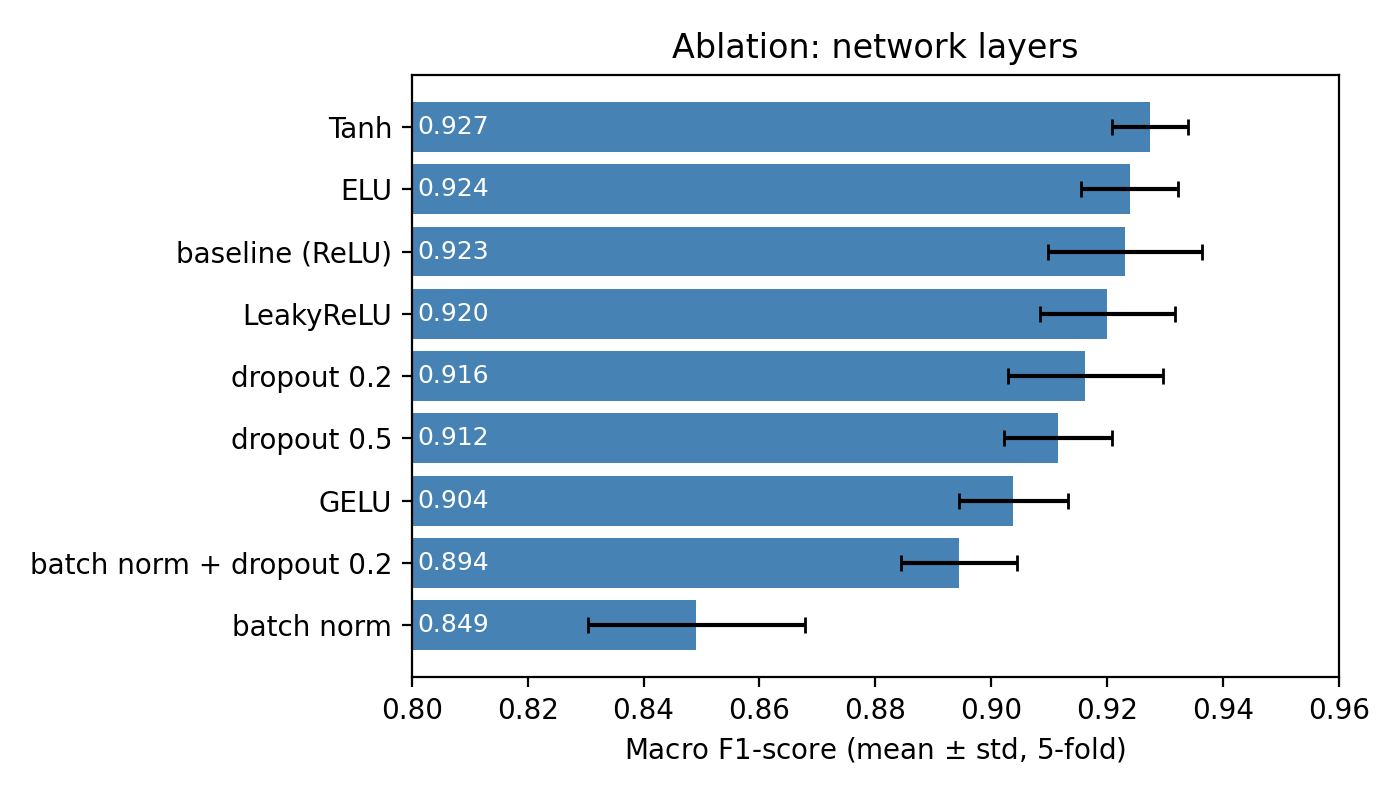
\includegraphics[width=\linewidth]{figures/ablation_layers.png}
        \end{column}
        \begin{column}{0.38\textwidth}
            \small
            Loss fixed to cross-entropy.
            \begin{itemize}
                \item Best: Tanh (0.927)
                \item ELU, ReLU, LeakyReLU are within one std of Tanh
                \item Dropout does not help
                \item Batch norm hurts the most (0.849)
            \end{itemize}
        \end{column}
    \end{columns}
\end{frame}

\begin{frame}
    \frametitle{Results Experiment: Loss Functions}
    \begin{columns}[c]
        \begin{column}{0.62\textwidth}
            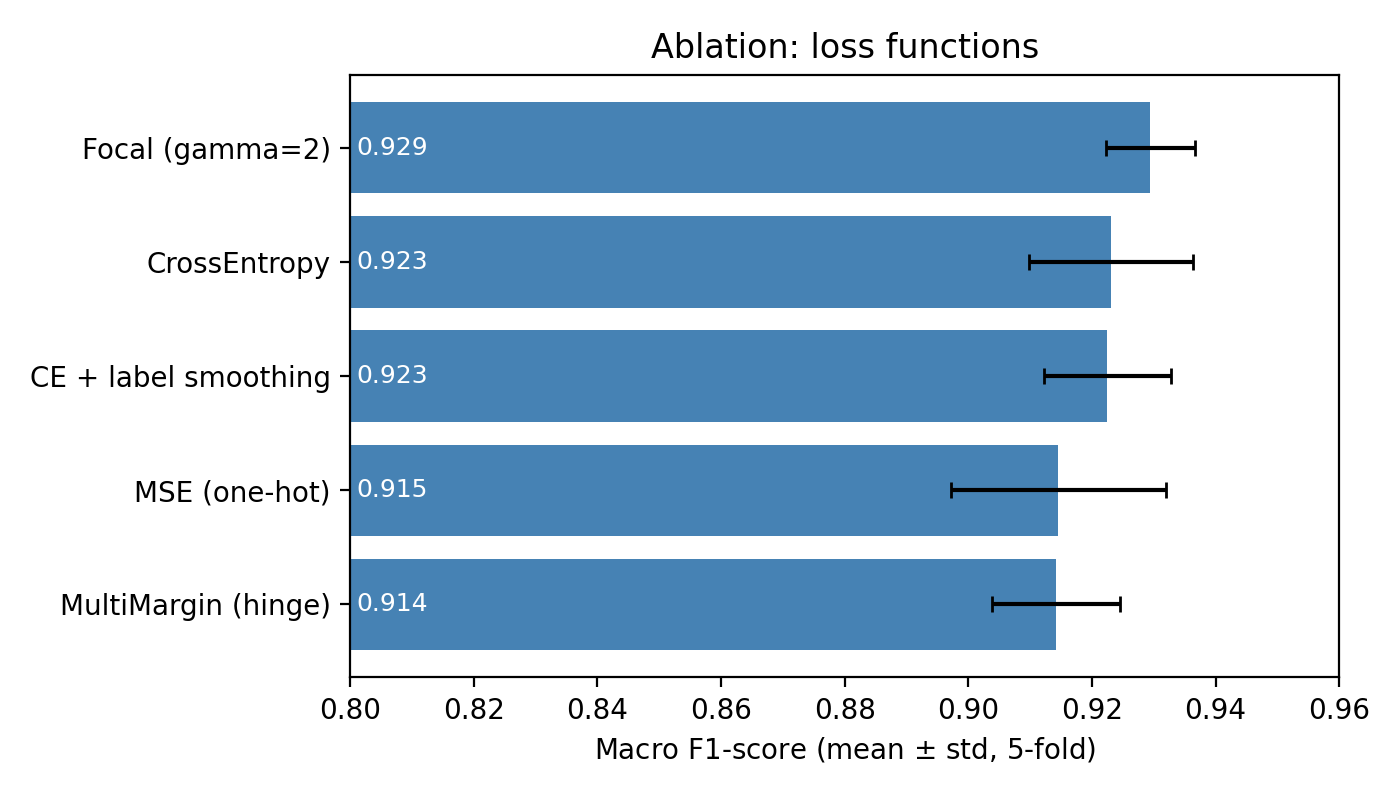
\includegraphics[width=\linewidth]{figures/ablation_loss.png}
        \end{column}
        \begin{column}{0.38\textwidth}
            \small
            Architecture fixed to baseline (ReLU, no dropout).
            \begin{itemize}
                \item Best: focal loss (0.930)
                \item Cross-entropy (0.923) and label smoothing (0.923) are similar
                \item Multi-margin and MSE are lower (0.914--0.915)
            \end{itemize}
        \end{column}
    \end{columns}
\end{frame}

\begin{frame}
    \frametitle{Results Experiment: Summary}
    \begin{columns}[c]
        \begin{column}{0.5\textwidth}
            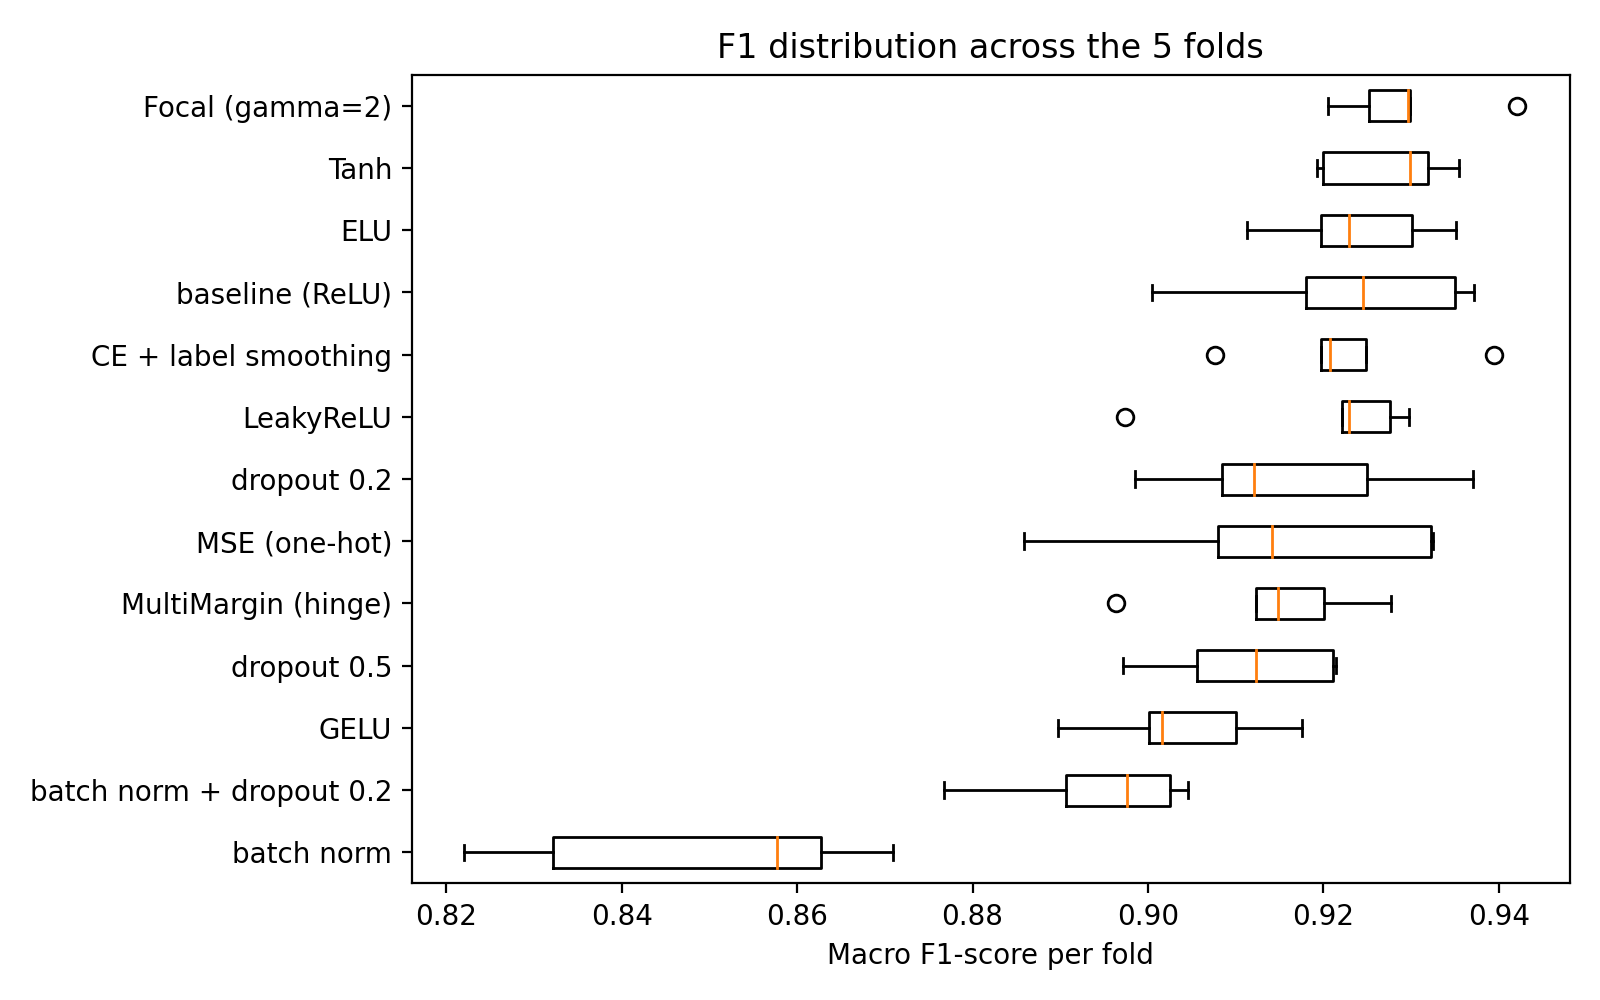
\includegraphics[width=\linewidth]{figures/fold_boxplot.png}
        \end{column}
        \begin{column}{0.5\textwidth}
            \footnotesize
            \begin{tabular}{lc}
                \toprule
                Experiment & F1 (mean $\pm$ std) \\
                \midrule
                Baseline (ReLU, CE) & 0.923 $\pm$ 0.013 \\
                Tanh & 0.927 $\pm$ 0.007 \\
                ELU & 0.924 $\pm$ 0.008 \\
                Dropout 0.2 & 0.916 $\pm$ 0.013 \\
                Batch norm & 0.849 $\pm$ 0.019 \\
                \midrule
                Focal loss & \textbf{0.930} $\pm$ 0.007 \\
                Label smoothing & 0.923 $\pm$ 0.010 \\
                Multi-margin & 0.914 $\pm$ 0.010 \\
                MSE (one-hot) & 0.915 $\pm$ 0.017 \\
                \bottomrule
            \end{tabular}
        \end{column}
    \end{columns}
\end{frame}

\begin{frame}
    \frametitle{Discussion}
    \begin{itemize}
        \item Most variants are within about one standard deviation of the baseline, so the differences among the top models are not clearly significant
        \item Dropout did not improve F1; with only 20 epochs the baseline is likely not overfitting enough to need extra regularization
        \item Batch norm clearly lowered F1 (0.849); adding dropout partly recovered it (0.894)
        \item Smooth activations (Tanh, ELU) are slightly better and more stable across folds than GELU
        \item Focal loss gave the highest mean F1 with a low std, but its gain over cross-entropy is small (about 0.007)
    \end{itemize}
\end{frame}

\begin{frame}
    \frametitle{Conclusion}
    \begin{itemize}
        \item An MLP reaches a macro F1-score of about 0.92--0.93 on mobile price range classification
        \item Best loss: focal loss (F1 $= 0.930$); best layer variant: Tanh activation (F1 $= 0.927$)
        \item Batch norm and, in this setup, dropout did not help
        \item Future work: combine the best layer and loss settings, tune the learning rate and number of epochs, and confirm on a held-out set
    \end{itemize}
\end{frame}

\begin{frame}
    \frametitle{GitHub Link}
    \url{https://github.com/yusufimantaka/mobile-price-range-classification}
\end{frame}

\begin{frame}[allowframebreaks]
    \frametitle{References}
    \footnotesize
    \begin{thebibliography}{9}
        \bibitem{kaggle} A.\ Sharma, ``Mobile Price Classification,'' Kaggle. \url{https://www.kaggle.com/datasets/iabhishekofficial/mobile-price-classification}
        \bibitem{pytorch} A.\ Paszke et al., ``PyTorch: An Imperative Style, High-Performance Deep Learning Library,'' NeurIPS, 2019.
        \bibitem{sklearn} F.\ Pedregosa et al., ``Scikit-learn: Machine Learning in Python,'' JMLR, vol.\ 12, 2011.
        \bibitem{adam} D.\ P.\ Kingma and J.\ Ba, ``Adam: A Method for Stochastic Optimization,'' ICLR, 2015.
        \bibitem{dropout} N.\ Srivastava et al., ``Dropout: A Simple Way to Prevent Neural Networks from Overfitting,'' JMLR, vol.\ 15, 2014.
        \bibitem{bn} S.\ Ioffe and C.\ Szegedy, ``Batch Normalization: Accelerating Deep Network Training by Reducing Internal Covariate Shift,'' ICML, 2015.
        \bibitem{focal} T.-Y.\ Lin et al., ``Focal Loss for Dense Object Detection,'' ICCV, 2017.
    \end{thebibliography}
\end{frame}
\end{document}
